\let\negmedspace\undefined
\let\negthickspace\undefined
\documentclass[journal]{IEEEtran}
\usepackage[a5paper, margin=10mm, onecolumn]{geometry}
%\usepackage{lmodern} % Ensure lmodern is loaded for pdflatex
\usepackage{tfrupee} % Include tfrupee package

\setlength{\headheight}{1cm} % Set the height of the header box
\setlength{\headsep}{0mm}     % Set the distance between the header box and the top of the text

\usepackage{gvv-book}
\usepackage{gvv}
\usepackage{cite}
\usepackage{amsmath,amssymb,amsfonts,amsthm}
\usepackage{algorithmic}
\usepackage{graphicx}
\usepackage{textcomp}
\usepackage{xcolor}
\usepackage{txfonts}
\usepackage{listings}
\usepackage{enumitem}
\usepackage{mathtools}
\usepackage{gensymb}
\usepackage{comment}
\usepackage[breaklinks=true]{hyperref}
\usepackage{tkz-euclide} 
\usepackage{listings}
% \usepackage{gvv}                                        
\def\inputGnumericTable{}                                 
\usepackage[latin1]{inputenc}                                
\usepackage{color}                                            
\usepackage{array}                                            
\usepackage{longtable}                                       
\usepackage{calc}                                             
\usepackage{multirow}                                         
\usepackage{hhline}                                           
\usepackage{ifthen}                                           
\usepackage{lscape}
\begin{document}

\bibliographystyle{IEEEtran}
\vspace{3cm}

\title{7-7.2-25}
\author{EE24BTECH11027 - satwikagv}
% \maketitle
% \newpage
% \bigskip
{\let\newpage\relax\maketitle}

\renewcommand{\thefigure}{\theenumi}
\renewcommand{\thetable}{\theenumi}
\setlength{\intextsep}{10pt} % Space between text and floats


\numberwithin{equation}{enumi}
\numberwithin{figure}{enumi}
\renewcommand{\thetable}{\theenumi}
\textbf{Question}:\\
Find the equation of a circle passing through the point \brak{7,3} having radius 3 units and whose centre lies on the line $y=x-1$.\\
\textbf{solution}:
\begin{table}[h!]    
  \centering
  \begin{tabular}[12pt]{ |c| c|}
    \hline
    \textbf{Variable} & \textbf{Description}\\ 
    \hline
    $P$ & point vector\\
    \hline 
    $-u$ & centre of the circle\\
    \hline
    $r$ & radius of the circle\\
    \hline 
    \end{tabular}

  \caption{Variables Used}
\end{table}
From the given information, the following equations can be formulated using the circle equation 
\begin{align}
\|x\|^2 + 2u^\top x + f &= 0\\
\|P\|^2 + 2u^\top P + f &= 0\\
\|u\|^2 - f &= r^2
\end{align}
From \brak{0.2} and \brak{0.3}
\begin{align}
\|P\|^2 + 2u^\top P + \|u\|^2 = r^2 	
\end{align}
Substituting the values of $u$,$p$ and $r$,
\begin{align}
k^2+(1-k)^2+2\myvec{-k&1-k}\myvec{7\\3}+\|P\|^2-r^2 = 0\\
2k^2-2k+1+6-20k+7^2+3^2-3^2=0\\
2k^2-22k+56=0\\
k=7,4
\end{align}
resulting in circles with centres 
\begin{align}
-u=\myvec{7\\6} or \myvec{4\\3}	
\end{align}
\begin{figure}[h!]
   \centering
   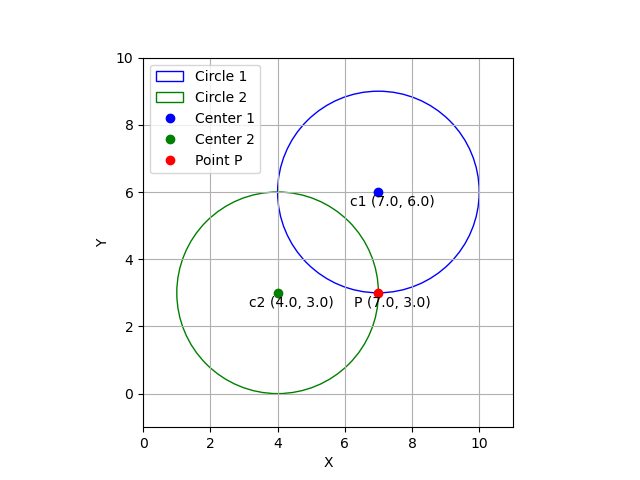
\includegraphics[width=0.7\linewidth]{figs/circle_plot.png}
   \caption{circles passing through point $\vec{P}\brak{7,3}$}
\end{figure}
\end{document}
